\documentclass[journal]{IEEEtran}

\usepackage{amsmath,amssymb,bm}
\usepackage{booktabs}
\usepackage{array}
\usepackage{cite}
\usepackage{microtype}
\usepackage{tikz}
\usepackage{xcolor}
\usepackage[hidelinks]{hyperref}
\usetikzlibrary{arrows.meta,calc,positioning,shapes.geometric}

\hypersetup{
  pdftitle={A Mathematical Specification for Multi-Image Projection, Alignment, Stereo Presentation, and Surface Reconstruction},
  pdfauthor={Sightline Technical Reference},
  pdfsubject={Implementation-independent geometry and conformance specification}
}

\newcommand{\R}{\mathbb{R}}
\newcommand{\T}{^{\mathsf T}}
\newcommand{\skewm}[1]{\left[#1\right]_{\times}}
\newcommand{\norm}[1]{\left\lVert #1\right\rVert}
\newcommand{\Exp}{\operatorname{Exp}}
\newcommand{\argmin}{\operatorname*{arg\,min}}
\newcommand{\diag}{\operatorname{diag}}
\newcommand{\med}{\operatorname{median}}
\newcommand{\trace}{\operatorname{tr}}
\newcommand{\code}[1]{\texttt{#1}}

\definecolor{specblue}{RGB}{28,91,153}
\definecolor{specorange}{RGB}{213,112,31}
\definecolor{specgreen}{RGB}{50,130,90}
\definecolor{specgray}{RGB}{90,96,104}

\title{A Mathematical Specification for Multi-Image Projection, Alignment, Stereo Presentation, and Surface Reconstruction}

\author{Sightline Technical Reference%
\thanks{Living technical specification, revision 1.0, July 2026. The equations are implementation independent; a direct double-precision procedural companion supplies executable conformance evidence.}}

\begin{document}
\maketitle

\begin{abstract}
This paper fixes the mathematical contract for a multi-image airborne imaging
system that supports planar projection, sparse and dense correspondence,
network attitude adjustment, uncertainty-aware reconstruction, surface
products, reference-terrain registration, and stereo presentation. The
specification separates physical geometry from plane-coordinate
reparameterization and display-only transforms. It defines right-handed frames,
full-source image coordinates, ray and plane equations, robust objectives,
pass-correlated priors, tangent-space time-varying research, dense matching,
multi-ray estimation, covariance, numerical precision, and degeneracy states.
A direct procedural two-image red/cyan path is specified as the executable
companion and first independent translation oracle. Detailed Jacobians,
multi-image normal equations, dense costs, and conformance rules appear in the
appendices.
\end{abstract}

\begin{IEEEkeywords}
photogrammetry, pushbroom imaging, bundle adjustment, stereo matching,
anaglyph, triangulation, uncertainty, digital elevation model, numerical
precision
\end{IEEEkeywords}

\section{Scope and Invariants}

\IEEEPARstart{T}{he} system considered here observes a physical scene from two
or more time-dependent viewpoints. A view can be a frame image, a line-scanner
product, or any source for which a continuous world ray can be formed at a
full-source image coordinate. Measurements may be inspected pairwise, but
accepted evidence belongs to one stable multi-image network. The mathematical
contract therefore centers stable view identity, explicit frames and units,
observable parameterizations, and immutable evidence generations.

Three kinds of transformation must remain distinct.
\begin{enumerate}
\item A \emph{physical transform} changes a source origin, a source ray, a
      terrain surface, or another quantity that affects scientific geometry.
\item A \emph{plane reparameterization} changes only the two basis vectors used
      to label points on an unchanged physical plane.
\item A \emph{presentation transform} changes only camera or display position,
      eye parallax, visibility, or color composition.
\end{enumerate}
Only the first category can change a reconstructed point or a backend scientific
product. This distinction prevents a visually useful stereo exaggeration from
being mistaken for a measurement correction.

All authoritative geometry, estimation, covariance, and procedural-reference
operations use IEEE 754 double precision. Full-source coordinates are ordered
as column then row, $\bm u=[c,r]\T$, although arrays are indexed by row then
column. Angles are radians and angular covariance is radians squared. Points and
vectors are columns. These choices follow established photogrammetric and
multiple-view practice \cite{Brown1971,HartleyZisserman2004,ForstnerWrobel2016}.

\begin{table*}[t]
\caption{Principal nomenclature. A subscript names a frame; $R_{ab}$ maps frame $b$ coordinates into frame $a$.}
\label{tab:nomenclature}
\centering
\footnotesize
\begin{tabular}{p{0.11\textwidth}p{0.35\textwidth}p{0.11\textwidth}p{0.31\textwidth}}
\toprule
Symbol & Meaning & Symbol & Meaning \\
\midrule
$W,E,B$ & World/project, local east-north-up, and platform body frames
& $G_r,G_p,S$ & Roll-gimbal, pitch-gimbal, and scanner frames \\
$\Pi,C,D$ & Physical plane, presentation camera, and display frames
& $I_i$ & Full-source image frame for stable view $i$ \\
$\bm p,\bm g,\bm v$ & World point, ray origin, and ray direction
& $\bm q=[x,y]\T$ & Coordinate in physical-plane basis $E_\Pi$ \\
$\bm u=[c,r]\T$ & Continuous full-source column/row coordinate
& $T_{ab},R_{ab},\bm t_{ab}$ & Homogeneous transform, rotation, and translation \\
$\bm\theta$ & Ordered omega, phi, kappa correction
& $\delta\bm\theta$ & Small local tangent rotation vector \\
$\bm b_{ij}$ & Baseline from view $i$ to view $j$
& $\rho,w$ & Robust loss and induced observation weight \\
$J,N,\Sigma$ & Jacobian, weighted normal matrix, and covariance
& $B_k(c),\bm a_{ik}$ & Cubic spline basis and tangent control vector \\
$d,\lambda$ & Disparity/search displacement and forward ray range
& $m$ & Explicit validity/evidence mask \\
\bottomrule
\end{tabular}
\end{table*}

\section{Frames, Transforms, and Sensor Formation}

\subsection{Rigid transforms and active rotations}

A right-handed rigid transform from frame $b$ to frame $a$ is
\begin{equation}
\bm p_a=R_{ab}\bm p_b+\bm t_{ab},\qquad
T_{ab}=\begin{bmatrix}R_{ab}&\bm t_{ab}\\\bm0\T&1\end{bmatrix}.
\label{eq:rigid}
\end{equation}
Composition follows the written frame chain, $T_{ac}=T_{ab}T_{bc}$. A small
active rotation $\delta\bm\theta$ left-composes a nominal attitude,
\begin{equation}
R^{+}=\Exp(\skewm{\delta\bm\theta})R^0,
\label{eq:leftcompose}
\end{equation}
where, for $a=\norm{\delta\bm\theta}$,
\begin{equation}
\Exp(\skewm{\delta\bm\theta})=I+
\frac{\sin a}{a}\skewm{\delta\bm\theta}+
\frac{1-\cos a}{a^2}\skewm{\delta\bm\theta}^2.
\label{eq:rodrigues}
\end{equation}
The series limit is used near zero. Equation~\eqref{eq:leftcompose} is also the
authoritative interpretation of an OPK increment: the named axes and order are
declared once, never inferred from storage order.

\subsection{Platform, gimbals, and line scanner}

At acquisition time $t$ and image column $c$, the source orientation is the
ordered chain
\begin{equation}
R_{WI}(t,c)=R_{WB}(t)R_{BG_r}(t)R_{G_rG_p}(t)
R_{G_pS}(t,c)R_{SI}.
\label{eq:sensorchain}
\end{equation}
The scanner term may vary by column. A body-frame lever arm $\bm\ell_B$ gives
the ray origin
\begin{equation}
\bm g_W(t,c)=\bm p_{WB}(t)+R_{WB}(t)\bm\ell_B.
\label{eq:lever}
\end{equation}
For calibrated image vector $\tilde{\bm u}$, the world ray is
\begin{equation}
\bm v_W(t,c,r)=
\frac{R_{WI}(t,c)K^{-1}\tilde{\bm u}}
{\norm{R_{WI}(t,c)K^{-1}\tilde{\bm u}}}.
\label{eq:rayformation}
\end{equation}
This model includes a linear pushbroom camera as a special case
\cite{GuptaHartley1997}. Timing, gimbal angle, lever arm, and calibration
provenance are distinct inputs; one must not absorb their errors into an
unlabeled image shift.

\begin{figure}[t]
\centering
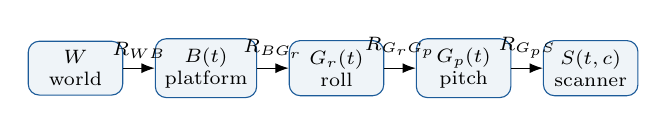
\begin{tikzpicture}[font=\scriptsize,node distance=4mm,>=Latex]
\tikzset{box/.style={draw=specblue,rounded corners,fill=specblue!7,
minimum width=12mm,minimum height=6mm,align=center}}
\node[box] (w) {$W$\\world};
\node[box,right=of w] (b) {$B(t)$\\platform};
\node[box,right=of b] (r) {$G_r(t)$\\roll};
\node[box,right=of r] (p) {$G_p(t)$\\pitch};
\node[box,right=of p] (s) {$S(t,c)$\\scanner};
\draw[->] (w)--node[above]{$R_{WB}$}(b);
\draw[->] (b)--node[above]{$R_{BG_r}$}(r);
\draw[->] (r)--node[above]{$R_{G_rG_p}$}(p);
\draw[->] (p)--node[above]{$R_{G_pS}$}(s);
\end{tikzpicture}
\caption{The platform-gimbal-scanner order is explicit. Reordering factors
changes the physical ray and is not a convention-only edit.}
\label{fig:sensorchain}
\end{figure}

\section{Physical Planes, Rays, and Full-Source Projection}

\subsection{Plane construction and coordinates}

A physical plane is
\begin{equation}
\Pi=\{\bm p:\bm p=\bm p_0+E_\Pi\bm q\},\qquad
E_\Pi=[\bm e_x,\bm e_y],
\label{eq:plane}
\end{equation}
with $E_\Pi\T E_\Pi=I_2$ and
$\bm e_x\times\bm e_y=\bm n$. Coordinates and reconstruction are
\begin{equation}
\bm q=E_\Pi\T(\bm p-\bm p_0),\qquad
\bm p=\bm p_0+E_\Pi\bm q.
\label{eq:planeroundtrip}
\end{equation}
Rotating $E_\Pi$ about $\bm n$ changes labels $\bm q$ but not $\Pi$. Tilting
$\bm n$ or moving $\bm p_0$ changes the physical plane. Ordered corners use a
declared clockwise or counterclockwise convention as viewed from $+\bm n$;
the order is never reconstructed from array position.

\subsection{Ray intersection}

For ray $\bm p(\lambda)=\bm g+\lambda\bm v$, intersection with $\Pi$ is
\begin{equation}
\lambda=\frac{\bm n\T(\bm p_0-\bm g)}{\bm n\T\bm v},\qquad
\bm p=\bm g+\lambda\bm v.
\label{eq:rayplane}
\end{equation}
The result is valid only when the denominator is separated from zero and
$\lambda>0$. Terrain intersection replaces the plane equation by a height or
implicit-surface residual and uses a bracketed or otherwise guarded root solve.
Voids, exclusions, horizon misses, and nonconvergence are named mask states.

\begin{figure}[t]
\centering
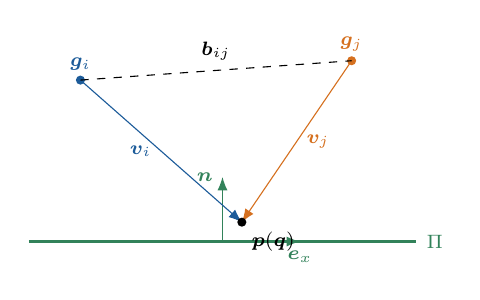
\begin{tikzpicture}[font=\scriptsize,scale=.82,>=Latex]
\coordinate (g1) at (-2.2,2.5); \coordinate (g2) at (2.0,2.8);
\coordinate (p) at (.3,.3);
\draw[thick,specgreen] (-3,0)--(3,0) node[right]{$\Pi$};
\draw[->,specgreen] (0,0)--(0,1.0) node[left]{$\bm n$};
\draw[->,specgreen] (0,0)--(1.2,0) node[below]{$\bm e_x$};
\fill[specblue] (g1) circle (2pt) node[above]{$\bm g_i$};
\fill[specorange] (g2) circle (2pt) node[above]{$\bm g_j$};
\draw[->,specblue] (g1)--(p) node[midway,left]{$\bm v_i$};
\draw[->,specorange] (g2)--(p) node[midway,right]{$\bm v_j$};
\fill[black] (p) circle (2pt) node[below right]{$\bm p(\bm q)$};
\draw[dashed] (g1)--(g2) node[midway,above]{$\bm b_{ij}$};
\end{tikzpicture}
\caption{A physical point is reconstructed from forward rays. The plane basis
labels the point but does not alter either source ray.}
\label{fig:rayplane}
\end{figure}

\subsection{Inverse mapping and resampling}

The backend mapping is output driven. Source rays sampled on a full-source mesh
produce pairs $(\bm q_{ik},\bm u_{ik})$. A continuous inverse map is
\begin{equation}
\bm u_i(\bm q)=\mathcal I_{\rm sc}
\left(\{\bm q_{ik}\mapsto\bm u_{ik}\},\bm q\right),
\label{eq:inversemap}
\end{equation}
where interpolation is undefined outside supported topology. Radiometry is then
sampled separately,
\begin{equation}
I_i^\Pi(\bm q)=\mathcal I_{\rm img}(I_i,\bm u_i(\bm q)),
\quad m_i=m_{\rm geom}m_{\rm image}m_{\rm operator}.
\label{eq:resampling}
\end{equation}
Nearest and bilinear sampling are explicit options. Invalid fill is an output
policy, never evidence. Display pyramids or preview tiles cannot replace the
full-source radiometric input.

\section{Sparse Correspondence and Track Evidence}

Feature detection and description create candidate observations with scale,
orientation, descriptor, mask, and source-coordinate provenance. Descriptor
distance, ratio, uniqueness, tie, texture, and radiometric compatibility remain
inspectable. Consensus fitting can use a similarity, affine, or other declared
image-space model under a robust sampling method such as RANSAC
\cite{FischlerBolles1981}; descriptor construction may follow established local
feature methods \cite{Lowe2004}.

For physically calibrated rays, a baseline-normalized coplanarity residual is
\begin{equation}
e_{ij}=\frac{(\bm v_i\times\bm v_j)\T\bm b_{ij}}
{\max(\norm{\bm b_{ij}},\epsilon_b)}.
\label{eq:coplanarity}
\end{equation}
This scalar triple product is invariant to a uniform baseline scale. Degenerate
baselines and invalid rays are reported, not assigned a small residual.

A track is a set of observations hypothesized to represent one physical point.
It contains at most one observation from each stable view. Direct and composed
paths are compared before merging; a cycle disagreement is diagnostic evidence,
not another independent solver residual. The pair graph first spans every
feasible connected component and then adds complementary loop chords only when
they improve conditioning or validate an independent path.

\begin{figure}[t]
\centering
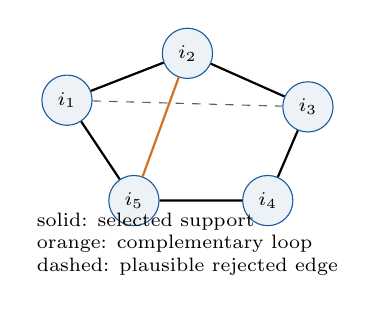
\begin{tikzpicture}[font=\scriptsize,>=Latex,scale=.85]
\foreach \x/\y/\n in {0/1.5/1,1.8/2.2/2,3.6/1.4/3,3.0/0/4,1.0/0/5}{
  \node[circle,draw=specblue,fill=specblue!8,minimum size=6mm] (v\n) at (\x,\y) {$i_\n$};}
\draw[thick] (v1)--(v2)--(v3)--(v4)--(v5)--(v1);
\draw[thick,specorange] (v2)--(v5);
\draw[dashed,specgray] (v1)--(v3);
\node[align=left] at (1.8,-.65) {solid: selected support\\orange: complementary loop\\dashed: plausible rejected edge};
\end{tikzpicture}
\caption{Measurements are generated pairwise but reconciled into one network.
Redundant pair multiplicity does not create independent physical evidence.}
\label{fig:network}
\end{figure}

\section{Global Attitude Adjustment}

\subsection{Robust objective, priors, and gauge}

Let $\bm\delta$ collect the active attitude increments. With residuals
$r_m(\bm\delta)$, standard deviations $\sigma_m$, and prior factor $L$, the
bounded objective is
\begin{equation}
\widehat{\bm\delta}=\argmin_{\bm\delta\in\mathcal B}
\sum_m \rho\!\left(\frac{r_m(\bm\delta)}{\sigma_m}\right)
+\norm{L(\bm\delta-\bm\mu)}^2.
\label{eq:networkobjective}
\end{equation}
Huber loss supplies an interpretable default robustifier
\cite{Huber1964}. Priors are outside observation robustification. Bounds are
physical safeguards, and a bound hit is a diagnostic rather than proof of
convergence.

Same-pass structure is
\begin{equation}
\delta\bm\theta_i=\delta\bm\theta_{p(i)}+\bm\epsilon_i,
\qquad \sum_{i\in p}\Lambda_i\bm\epsilon_i=\bm0,
\label{eq:passmodel}
\end{equation}
where the second relation is a precision-weighted balanced gauge. Independent
passes have separate common terms and are connected only by cross-pass evidence
or an explicit prior. Silently fixing the first view is prohibited because it
concentrates gauge uncertainty in an arbitrary observation.

At a linearization point,
\begin{equation}
N=J\T WJ+L\T L,\qquad
\Sigma_{\delta}=N^{\dagger},
\label{eq:normal}
\end{equation}
only when rank, gauge, and conditioning justify covariance. The decomposition
of data and prior objective, connected components, weak views, leave-one-edge
sensitivity, and residual summaries by pass, time, and image region remain
reported. This is the sparse block structure familiar from bundle adjustment
\cite{Triggs2000}.

\subsection{Time-varying attitude research}

After a constant solution, a bounded research model represents within-image
attitude by local rotation vectors,
\begin{equation}
\delta\bm\theta_i(c)=\delta\bm\theta_{p(i)}+
\sum_k B_{ik}(c)\bm a_{ik},
\label{eq:splineattitude}
\end{equation}
where $B_{ik}$ are open-uniform cubic B-splines initially spaced every 128
full-source columns \cite{DeBoor2001}. Each attitude is composed through
\eqref{eq:leftcompose}; Euler angles are never interpolated. A second-difference
penalty $\sum_i\norm{D_2\bm a_i}^2$ supplies smoothness, and the differential
controls retain a balanced pass gauge.

Post spacing doubles until local support, data rank, and condition are adequate,
or until a declared maximum proves the model insufficient. A one-column model
is only an upper-bound experiment. Synthetic algebraic recovery does not prove
physical observability, so time-varying corrections remain review-only until
held-out physical evidence establishes stability and value beyond the constant
model.

\section{Pair Camera and Stereo Presentation}

\subsection{Pair viewpoint}

A pair camera is a presentation object. Its target is the common-footprint
centroid and its view direction points from a representative midpoint-derived
camera position toward that target. The camera up vector is derived from the
physical plane. Fitting, following, panning, zooming, and twisting do not change
the plane, rays, matches, or reconstructed products.

\subsection{Physical eye assignment with hysteresis}

Let $\bm r_C$ be camera right and $\bm g_i$ representative source origins. The
screen-horizontal positions are $s_i=\bm r_C\T\bm g_i$. Outside a normalized
head-on threshold $h$, the smaller $s_i$ is physical left and maps to red. If a
previous assignment exists, it switches only when
\begin{equation}
\frac{s_{\rm previous\ right}-s_{\rm previous\ left}}
{\norm{\bm g_2-\bm g_1}}<-h.
\label{eq:hysteresis}
\end{equation}
At an initially degenerate baseline, stable identity supplies the deterministic
tie break. A manual swap is presentation state and never rewrites view identity.

\subsection{Display-only parallax and red/cyan composition}

For view width $W_C$, exaggeration $\eta$, base fraction $\beta$, and screen
depth offset $d_0$, define
\begin{equation}
\Delta=(\eta-1)\beta W_C+d_0,\qquad
\bm o_L=-\Delta\bm r_C,\quad \bm o_R=+\Delta\bm r_C.
\label{eq:parallax}
\end{equation}
These offsets translate displayed eye surfaces only. On a fixed output plane,
the equivalent inverse sampling query is
\begin{equation}
\bm q_i^D=\bm q-E_\Pi\T\bm o_i.
\label{eq:displayquery}
\end{equation}
The physical $\bm q$, $\bm p$, plane, and source mesh remain unchanged. With
unit grayscale $Y_L,Y_R$ and common mask $m=m_Lm_R$, the canonical companion
anaglyph is
\begin{equation}
A(\bm q)=\left[Y_L(\bm q),Y_R(\bm q),Y_R(\bm q)\right],\quad m=1,
\label{eq:anaglyph}
\end{equation}
and explicit fill otherwise.

\begin{figure}[t]
\centering
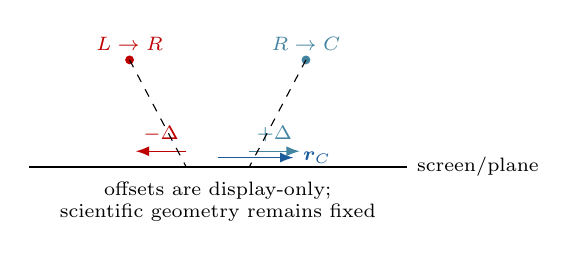
\begin{tikzpicture}[font=\scriptsize,scale=.8,>=Latex]
\draw[thick] (-3,0)--(3,0) node[right]{screen/plane};
\draw[->,specblue] (0,.15)--(1.2,.15) node[right]{$\bm r_C$};
\fill[red!75!black] (-1.4,1.7) circle (2pt) node[above]{$L\to R$};
\fill[cyan!60!black] (1.4,1.7) circle (2pt) node[above]{$R\to C$};
\draw[->,red!75!black] (-.5,.25)--(-1.3,.25) node[midway,above]{$-\Delta$};
\draw[->,cyan!60!black] (.5,.25)--(1.3,.25) node[midway,above]{$+\Delta$};
\draw[dashed] (-1.4,1.7)--(-.5,0);
\draw[dashed] (1.4,1.7)--(.5,0);
\node[align=center] at (0,-.55) {offsets are display-only;\\scientific geometry remains fixed};
\end{tikzpicture}
\caption{Physical eye identity controls color; symmetric display translations
control perceived separation and depth.}
\label{fig:stereo}
\end{figure}

\section{Dense Correspondence}

Dense processing is planned independently of the sparse alignment graph. Pair
selection considers overlap, intersection angle, texture, radiometry,
visibility, conditioning, expected work, and validation views. Sparse tracks
may seed local disparity or direction priors, but unsupported regions remain
explicitly unseeded rather than inheriting fabricated depth.

For zero-mean patches $a,b$, a common normalized cost is
\begin{equation}
C_{\rm ZNCC}=1-\frac{a\T b}{\norm{a}\norm{b}}.
\label{eq:zncc}
\end{equation}
Gradient, census/rank, and phase-only costs are separate declared alternatives.
Uniqueness, ties, low texture, prediction residual, and forward/backward
consistency remain state evidence. If $C_{-},C_0,C_{+}$ bracket a strict local
minimum, bounded parabolic refinement gives
\begin{equation}
d^*=d_0+\frac{C_{-}-C_{+}}
{2(C_{-}-2C_0+C_{+})}.
\label{eq:subpixel}
\end{equation}
Left/right consistency rejects or labels an observation when
$\norm{\bm u_L-FB(\bm u_L)}>\tau_{FB}$. Semi-global matching is retained as a
classical baseline, not an automatic universal choice
\cite{Hirschmuller2008,ScharsteinSzeliski2002}.

\begin{figure}[t]
\centering
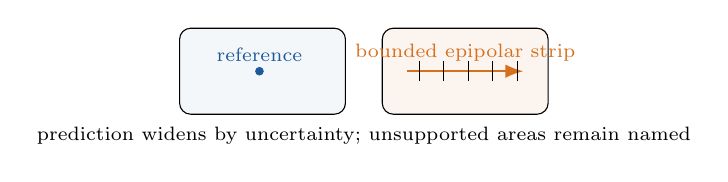
\begin{tikzpicture}[font=\scriptsize,scale=.78,>=Latex]
\draw[rounded corners,fill=specblue!5] (-3,-.7) rectangle (-.3,.7);
\draw[rounded corners,fill=specorange!7] (.3,-.7) rectangle (3,.7);
\fill[specblue] (-1.7,0) circle (2pt) node[above]{reference};
\draw[specorange,thick,->] (.7,0)--(2.6,0) node[midway,above]{bounded epipolar strip};
\foreach \x in {.9,1.3,1.7,2.1,2.5}{\draw (\x,-.16)--(\x,.16);}
\node at (0,-1.05) {prediction widens by uncertainty; unsupported areas remain named};
\end{tikzpicture}
\caption{Dense search is bounded by geometry and uncertainty, then audited by
uniqueness, texture, and bidirectional consistency.}
\label{fig:dense}
\end{figure}

\section{Triangulation, Uncertainty, and Surface Products}

\subsection{Pairwise and robust multi-ray reconstruction}

Given unit rays $(\bm g_i,\bm v_i)$, the linear multi-ray point minimizes
orthogonal ray distance,
\begin{equation}
\widehat{\bm p}=\argmin_{\bm p}
\sum_i w_i\norm{(I-\bm v_i\bm v_i\T)(\bm p-\bm g_i)}^2.
\label{eq:multiray}
\end{equation}
Weights are robust and equalized by unique view/pass evidence; pair
multiplicity cannot increase independent support. Forward range, ray angle,
normal rank, condition, residual, radiometry, visibility, and rejected-ray
provenance determine reliability. Two-view triangulation is the labeled special
case discussed by Hartley and Sturm \cite{HartleySturm1997}. Competing depth
modes remain separate when the evidence supports more than one surface.

\subsection{Covariance}

With observation coordinates $\bm u$, source-state variables $\bm s$, and
linearization Jacobians $J_u,J_s$,
\begin{equation}
\Sigma_p=J_u\Sigma_uJ_u\T+J_s\Sigma_sJ_s\T
+J_u\Sigma_{us}J_s\T+J_s\Sigma_{us}\T J_u\T.
\label{eq:pointcov}
\end{equation}
Correlation terms are retained when errors share navigation, pass, or DEM
sources. Numerical Jacobians use scale-aware perturbations and symmetry checks;
analytic forms are preferred at frozen high-value kernels. An unavailable or
rank-deficient covariance is labeled rather than replaced with zeros.

\subsection{Fusion and surface formation}

The authoritative point product preserves every contributing source
observation and its full-source coordinate. Optional occupancy, Gaussian,
mesh, and grid products are estimators over this evidence, not replacements for
it. Sparse occupancy votes, uncertainty-aware splats, and direct multi-ray
points can be compared over GSD-derived scale sweeps. A surface product records
resolution, mask, uncertainty, contributing views/passes, competing modes,
decimation, and whether it is authoritative or diagnostic.

\section{Reference Terrain Registration}

A terrain grid declares horizontal datum, vertical datum, units, accuracy,
voids, masks, and transformations between geodetic, local ENU, and project
world coordinates. A robust translation-only registration uses reference
points $\bm d_k$ and normals $\bm n_k$,
\begin{equation}
\widehat{\bm t}=\argmin_{\bm t}\sum_k
\rho\!\left(\frac{\bm n_k\T(\bm p_k+\bm t-\bm d_k)}{\sigma_k}\right).
\label{eq:demobjective}
\end{equation}
The normal matrix includes point covariance, local terrain uncertainty, and a
shared DEM error floor. Flat or weakly distributed terrain produces an
ambiguity state. Buildings, water, voids, and caller exclusions remain named
mask evidence. The method relates to point/surface registration principles
\cite{BeslMcKay1992,Censi2007}, but application is an explicit, atomic, and
revertible physical source-origin change. Imagery-only points remain preserved
for comparison.

\section{Numerical Precision and Conformance}

Large world coordinates can destroy small baselines if cast before local
subtraction. The safe display boundary is
\begin{equation}
\bm p_{\rm local}^{(d)}=\bm p_W^{(d)}-\bm o_W^{(d)},\qquad
\bm p_{\rm display}^{(s)}=\operatorname{single}(\bm p_{\rm local}^{(d)}),
\label{eq:precision}
\end{equation}
where superscripts identify double and single. Absolute world positions, ray
intersection, inverse mapping, alignment, covariance, triangulation, and the
procedural reference remain double. Dense costs or discardable display
coordinates may use an explicit mixed boundary only after comparison with the
double path.

Golden acceptance combines absolute, relative, angular, pixel, and mask terms.
Every result records algorithm/version, precision, frame, units, input
fingerprint, capability/fallback, deterministic options, and timing. A completed
result must be invariant to cancellation polling and progress reporting.
Independent ports compare plane/world coordinates, continuous source maps,
values, masks, eye identity, presentation offsets, and stereo composition.
Matrix rank and conditioning follow stable numerical linear algebra practice
\cite{GolubVanLoan2013}.

\section{Limitations and Degeneracies}

The model cannot recover information absent from the observations. Named stop
or review states include parallel or behind-origin rays; empty or unverifiable
source support; duplicate identities; feature ties; repeated or textureless
regions; disconnected or ungauged networks; weak rank or condition; bound hits;
prior-dominated attitude; near-parallel triangulation; competing depth modes;
terrain voids and datum ambiguity; and unavailable covariance. Presentation
quality does not override these states.

Atmospheric refraction, rolling-shutter effects beyond the declared source
model, cloud/water semantic screening, high-order calibration drift, and
production time-varying attitude remain outside the authoritative scope until
their parameters and observability are approved. GPU and lower-precision paths
are optional accelerators. They cannot remove the CPU double reference or its
error and mask semantics.

\appendices

\section{Rotation and Intersection Jacobians}

For $R^+=\Exp(\skewm{\delta\bm\theta})R$ near zero and fixed vector $\bm x$,
\begin{equation}
\frac{\partial(R^+\bm x)}{\partial\delta\bm\theta}\bigg|_{\bm0}
=-\skewm{R\bm x}.
\label{eq:rotjac}
\end{equation}
For the plane range in \eqref{eq:rayplane}, define
$a=\bm n\T(\bm p_0-\bm g)$ and $b=\bm n\T\bm v$. Then
\begin{equation}
\frac{\partial\lambda}{\partial\bm g}=-\frac{\bm n\T}{b},\qquad
\frac{\partial\lambda}{\partial\bm v}=-\frac{a}{b^2}\bm n\T,
\label{eq:rangejac}
\end{equation}
and
\begin{equation}
\frac{\partial\bm p}{\partial\bm g}=I+
\bm v\frac{\partial\lambda}{\partial\bm g},\quad
\frac{\partial\bm p}{\partial\bm v}=\lambda I+
\bm v\frac{\partial\lambda}{\partial\bm v}.
\label{eq:pointjac}
\end{equation}
The factors expose the $1/b$ and $1/b^2$ growth near parallel incidence. Such
geometry must be rejected or downweighted before covariance is interpreted.

\section{Network Linearization and Observability}

At iteration $k$, robust weights are frozen while solving
\begin{equation}
\begin{bmatrix}W^{1/2}J\\L\end{bmatrix}\Delta\bm\delta
=-\begin{bmatrix}W^{1/2}\bm r\\L(\bm\delta_k-\bm\mu)\end{bmatrix}.
\label{eq:augmented}
\end{equation}
The data-only singular spectrum diagnoses observation geometry; the augmented
spectrum diagnoses the numerical solve. A full augmented rank does not make an
unobservable data mode observable: it may only show that a prior filled that
mode. Reports therefore distinguish data rank, required gauge-adjusted rank,
augmented rank, data condition, prior contribution, and prior dominance.

For time-varying controls, each observation row contains a pass-common block and
at most four nonzero cubic basis blocks for its view. Coarsening reduces control
count and increases support. Promotion requires held-out physical improvement,
stable estimates under spacing perturbation, and an explicit source-geometry
application contract.

\section{Dense Cost and Consistency Details}

For patches $a,b$ with means $\bar a,\bar b$, ZNCC uses
\begin{equation}
\operatorname{ZNCC}(a,b)=
\frac{(a-\bar a\bm1)\T(b-\bar b\bm1)}
{\norm{a-\bar a\bm1}\norm{b-\bar b\bm1}}.
\end{equation}
A gradient cost applies a robust norm to horizontal/vertical derivative
differences. Census/rank costs compare local order bit strings by Hamming
distance. Phase-only cost normalizes cross-power magnitude before inverse
transformation. Constant patches, zero denominators, saturated neighborhoods,
and masks produce explicit states.

The subpixel denominator in \eqref{eq:subpixel} must indicate positive
curvature and the offset must stay within a declared interval, normally one
pixel. Forward/backward consistency is evaluated in continuous full-source
coordinates. Chunked implementations include search and interpolation halos so
interior results are independent of chunk boundaries.

\section{Multi-Image Association, Fusion, and Registration}

Dense pair observations are reconciled by stable view identity before 3-D
formation. A valid association has at most one observation per view; a conflict
cannot be hidden by pair order. The normal matrix for \eqref{eq:multiray} is
\begin{equation}
H=\sum_i w_i(I-\bm v_i\bm v_i\T),\qquad
\bm h=\sum_i w_i(I-\bm v_i\bm v_i\T)\bm g_i,
\end{equation}
with $H\widehat{\bm p}=\bm h$. Robust iteration updates residual weights while
keeping unique view/pass accounting. The eigenstructure of $H$ exposes weak
ray geometry.

Surface fusion retains a reverse link from every output element to contributing
points and source observations. DEM registration keeps vertical datum and
frame transformations outside the optimizer. For translation-only registration,
row $k$ of $J$ is $\bm n_k\T$; a flat normal distribution makes horizontal
translation weak regardless of point count. A shared DEM uncertainty component
sets a covariance floor that cannot be averaged away as independent noise.

\section{Procedural Two-Image Companion}

The executable companion accepts two in-memory image arrays, one physical
plane, camera values, two source-geometry functions, and explicit output and
stereo options. Its visible order is:
\begin{enumerate}
\item create the output grid in $\bm q$ and reconstruct $\bm p$;
\item derive camera right and assign physical eyes;
\item form symmetric display-only offsets using \eqref{eq:parallax};
\item intersect each source ray mesh with the physical plane;
\item construct the continuous inverse maps in \eqref{eq:inversemap};
\item query at \eqref{eq:displayquery}, sample full-source radiometry, and mask;
\item compose \eqref{eq:anaglyph}; and
\item return double values and portable explanatory metadata.
\end{enumerate}
It has no graphics, object hierarchy, hidden state, cache, tile pool, or implicit
cast. Runtime source functions are not retained in output. Golden tests compare
the direct algebra against production components rather than calling those
components from inside the companion.

\section{Cross-Language Conformance Matrix}

An implementation is conformant only when it passes the following layers:
\begin{enumerate}
\item frame, plane, ray, and inverse-map unit fixtures;
\item procedural two-image value, coordinate, mask, eye, and stereo fixtures;
\item sparse association and robust network fixtures, including degeneracy;
\item dense cost, subpixel, consistency, and chunk-boundary fixtures;
\item pair and multi-ray point/covariance fixtures;
\item surface and DEM registration fixtures; and
\item scale/precision fixtures through the required long-range geometry.
\end{enumerate}
Each record names compiler/runtime, hardware, precision, acceleration, input
fingerprint, tolerance, value error, mask mismatch, deterministic repeatability,
and timing. Passing compilation or visual similarity alone is insufficient.

\bibliographystyle{IEEEtran}
\bibliography{references}

\end{document}
